\item Due segmenti AB e BC sono disposti come in figura. Se AB è lungo 8 cm e BC è lungo 4 cm, che operazione fai per calcolare la lunghezza di AC?
\begin{figure}[h]
\centering
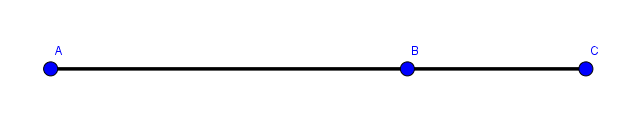
\includegraphics[width=13cm]{figure/somma_diff_segmenti.PNG}
\end{figure}
